%\begin{savequote}[8cm]
%Alles Gescheite ist schon gedacht worden.\\
%Man muss nur versuchen, es noch einmal zu denken.

%All intelligent thoughts have already been thought;\\
%what is necessary is only to try to think them again.
 % \qauthor{--- Johann Wolfgang von Goethe \cite{von_goethe_wilhelm_1829}}
%\end{savequote}

\chapter{\label{ch-FurtherSims} Further simulation campaigns in the low-CR regime}

\minitoc

\section{Introduction}
The previous chapter presented three key results. Firstly, the new low-instability regime was defined, where 1D simulations are expected to provide a reasonable estimate of performance. Secondly, the performance of conventional central hot-spot implosions of wetted-foam capsules using third-harmonic laser light in this regime was explored and well-characterised. Finally, the methodology for this style of optimisation campaign (and the necessary code to produce and analyse the simulations) was established.

In this chapter, these previous results are expanded in a variety of ways.  In Section \ref{sec:MixedEOS}, the impact of the EOS model used to describe the wetted-foam is investigated, in an attempt to address one of the major limitations of the previous campaign. One of the other limitations of this approach was the difficulty of verifying this regime experimentally, and so in Section \ref{sec:Hydroequivalent} new surrogate targets (`hydrodynamic equivalent' capsules) are proposed and optimised to enable room temperature experiments.

In the second half of the chapter, two further simulation campaigns are performed. In Section \ref{sec:AlternativeDrivers} the potential performance benefits of using higher frequency lasers are investigated, through additional implosion optimisations. Finally, in Section \ref{sec:AuxiliaryHeating}, an auxiliary heating scheme using electron beams is discussed and applied to these implosions. These campaigns further explore the possible performance of wetted-foam capsules within the low-instability regime, while also allowing the benefits of these alternative approaches to be assessed (through comparison with the results of the previous simulations).

\subsection{An alternative fusion metric: the burning plasma parameter}
It is useful at this stage to introduce an additional fusion metric, which will be used later in this chapter to evaluate fusion performance. So far in this thesis gain has been the primary fusion metric, but calculating gain requires the input energy of the implosion to be known. This is not the case in Section \ref{sec:AuxiliaryHeating}, due to uncertainty in the exact energy required to drive the auxiliary heating. This dependence on input energy means that the gain in this case is highly affected by `up-stream' efficiencies (such as how efficiently electron beams can be generated), and thus it is useful to use alternative metrics which do not share this dependence.

A metric known as the `burning plasma parameter' is therefore introduced for this chapter. The version used here - the `total capsule burning plasma parameter' - is defined as 
\begin{equation} Q^\mathrm{{tot}}_{\mathrm{\alpha}} = \frac{1}{2} \frac{E_\mathrm{\alpha}}{ E^\mathrm{{tot}}_{\mathrm{PdV}}}, \label{eqn:Qtot defn} \end{equation} where $E_\mathrm{\alpha}$ is the alpha particle energy deposited back into the hotspot over the total duration of the implosion, and $E^\mathrm{{tot}}_{\mathrm{PdV}}$ is the total work done on the capsule hotspot and shell until stagnation (the time of maximum pressure) \cite{Betti2015}. This metric compares the energy absorbed from alpha self-heating at the bang-time of the capsule, to the external energy that was used to compress it\footnote{The burn is assumed to be symmetric around the bang time, such that the alpha self-heating at the bang time is equal to half of the total alpha heating experienced over the full implosion, $E_\mathrm{\alpha}$. This is the source of the factor of half in the equation.}.

A value of $Q^\mathrm{{tot}}_{\mathrm{\alpha}} > 1$ defines the `burning plasma' regime, where alpha heating is the dominant source of energy in the capsule \cite{Christopherson2020}. The burning plasma parameter is therefore a useful metric for fusion capsules, as it provides direct information about the degree to which fusion reactions are contributing to the energetics of the hotspot. It does not depend on input energy, and thus how efficiently the capsule is driven; this makes it ideal for analysing the auxiliary heating simulations.

Previous works have also attempted to define ignition using such parameters. An early rough definition used an ignition threshold of $Q^\mathrm{{tot}}_{\mathrm{\alpha}} = 10$, defining ignition simply as when the self-heating was ten times greater than the work done on the hot spot and shell \cite{Betti2011}. Recently more rigorous definitions have been created, based instead on an alternative `hotspot burning plasma parameter', where the total work done on the whole capsule $E^\mathrm{{tot}}_{\mathrm{PdV}}$ is instead replaced by the total work done on the hotspot only. This quantity is typically twice as large as the `total capsule' version used in this thesis \cite{Betti2015}. Analysis of a number of simulations has led to an ignition criteria of  $Q^\mathrm{{hs}}_{\mathrm{\alpha}} > 1.4$ \cite{Christopherson2020} (where ignition here describes the point at which self-heating results in burn propagation through the cold shell).

\section{Estimating the impact of the wetted-foam EOS} \label{sec:MixedEOS}

The HYADES simulations used in this thesis are intended to describe wetted-foam targets, but the wetted-foam layer in these simulations is described using the pure-DT equation of state. This approximation does not account for the presence of the foam material, and was highlighted as a limitation of this work in the previous chapter. There is no wetted-foam equation of state that is currently generally available. Other work (at US national labs) has used a mixed equation of state, which does include the presence of the foam \cite{Olson2021}; this is reported to be less compressible than pure-DT, resulting in a thicker but less dense shell and a reduced fusion yield \cite{Olson2020a}.

The impact of using a more physical `mixed' equation of state was investigated using the alternative 1D radiation-hydrodynamic code HELIOS \cite{MacFarlane2006}. HELIOS is compatible with another program, PropacEOS, which is used to generate custom EOS tables for materials based on their atomic composition; these can then be used for HELIOS simulations involving these materials. A mixed-EOS table was produced for the wetted-foam in PropacEOS, assuming that it consisted of a 2\% atomic fraction of carbon, 48\% tritium, and 50\% deuterium (corresponding to a 25 \unit{\milli\gram\per\centi\meter\cubed} deuterated plastic foam, saturated with a 50:50 mix of liquid DT). 

HELIOS does not model the absorption of alpha-particles, which means that alpha self-heating is not described. This means that as implosions approach ignition (and self-heating begins to add substantial amounts of energy to the hotspot), the results will diverge from codes such as HYADES which do model these effects. To mitigate for this, the 0.25 size capsule was chosen for the comparison; the effects of self-heating will be minimal for such a capsule, and thus HELIOS can still be used to determine gain with reasonable accuracy.

Two HELIOS simulations using PropacEOS models were performed. The first used a pure-DT EOS to describe the foam layer, while the second used the new mixed EOS. Both simulations were otherwise unchanged (in terms of laser and capsule properties) from the HYADES simulation. Some differences are expected when changing between codes and EOS models, and so the pure-DT HELIOS simulation allowed these changed to be identified, and provided a better comparison with the mixed EOS results. The temperatures and densities achieved at the bang-time in the one HYADES and two HELIOS simulations are displayed in Figure \ref{fig:MixedEOS}, while the implosion parameters are displayed in Table \ref{tab:MixedEOS}.

\begin{figure} 
	\centering     %%% not \center
	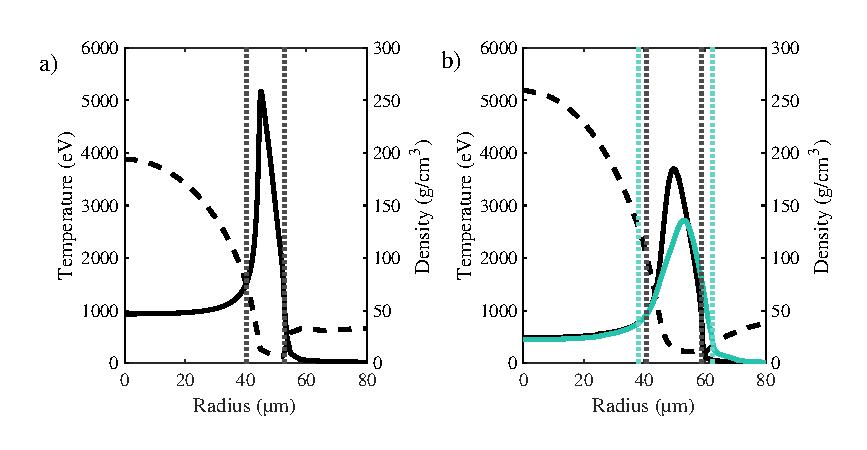
\includegraphics[width=.8\textwidth]{figures/FurtherSims/MixedEOS.eps}
	\caption{\label{fig:MixedEOS} Temperature (dashed lines) and density (solid line) at the bang time for a) the 0.25 size 4-pulse implosion simulated in HYADES, and b) the same simulation in HELIOS. In b), the teal solid line represents the density profile for the same simulation when a mixed-EOS is used (the temperature profiles for these two simulations overlap). The dotted vertical lines show the hotspot and shell boundaries (where again, the dotted teal lines refer to the mixed-EOS). )}
\end{figure}

\begin{table}
	\centering
	\begin{tabular}{|c|c|c|c|}
		\hline
		Code &  HYADES & HELIOS & HELIOS \\ 
		\hline
		EOS & Pure DT & Pure DT & Mixed \\
		\hline
		%Vapour density (\unit{\milli\gram\per\centi\meter\cubed}) & 1.35 & 1.35 & 1.35 \\
		Gain & 0.030 & 0.040 & 0.028  \\
		Convergence Ratio & 15.7 & 16.6 & 25.3 \\ 
		IFAR & 23.4 & 24.6 & 24.8 \\ 
		Implosion velocity (km/s) & 391.4 & 393.8 & 391.9 \\
		\hline
	\end{tabular}
	\caption{Simulation outputs for the same 0.25 simulations simulated in HYADES with a pure-DT EOS, and in HELIOS with both a pure-DT and a mixed-EOS.}
	\label{tab:MixedEOS}
\end{table}

Differences are seen between the pure-DT simulations in the two codes; the temperature in HELIOS is higher while the densities of both shell and hotspot are lower, and this results in a higher gain and a higher convergence ratio. The hydrodynamic behaviour is otherwise similar. Such differences are expected between different codes and methods for calculating EOS tables. Comparing the two HELIOS simulations, it can be seen that the mixed EOS is less compressible and results in a lower peak density and a thicker shell. The temperature profile is essentially unchanged when changing from pure-DT to mixed EOS. These results show good qualitative agreement with the mixed EOS results presented by Olson \textit{et al.} \cite{Olson2020a}.

The IFAR and implosion velocity using the mixed-EOS are similar to the pure-DT simulation, but the convergence ratio in Table \ref{tab:MixedEOS} is significantly higher. This is a consequence of the particular definition used to identify the hotspot radius\footnote{As the peak density is lower, the $1/e^2$ threshold used to define the hotspot occurs at a lower radius.}, rather than representing a physical change in the compression. It can be seen in Figure \ref{fig:MixedEOS} that the peak density for the mixed EOS simulation actually occurs at a greater radius, and the temperature profile (which was used in \cite{Olson2020a} to define convergence ratio) is unchanged between the two simulations. The increase in convergence ratio reported in in Table \ref{tab:MixedEOS} is thus not thought to be significant.

The use of a mixed-EOS table has reduced the gain to roughly 70\% of that obtained in the pure-DT simulation. It is difficult to extrapolate these results to larger capsules, as the self-heating instability could mean this results in even lower gains. However, the pure-DT implosion presented by Olson \textit{et al.} \cite{Olson2020a} had substantially greater fusion performance (with a 100 MJ yield), and a similar 30\% reduction was observed (with 71~MJ achieved using the mixed-EOS). This agreement is encouraging, and suggests that as a first estimate a yield reduction of 30\% may be expected when switching from a pure-DT to mixed EOS description of wetted-foam layers.

The comparison performed here is by no means definitive. It would be preferable to estimate the mixed EOS impact in HYADES directly, given that this is where the main campaign were performed. The PropacEOS tables were converted for use in HYADES, but physical results were not obtained when they were used in simulations\footnote{Such simulations showed an unphysical amount of ablation of shell material into the hotspot, reducing the temperature and significantly impacting the yield/gain. This appears to be a problem with the conduction model in HYADES, and is currently under investigation.}. This topic should be investigated further. Ultimately, mixed-EOS tables which describe wetted-foams should be produced and made publicly available, and wetted-foam EOS experiments should be performed to allow the accuracy of such models to be tested and verified.


%First, the four-pulse 0.25 size design (presented in Table \ref{tab:ThirdHarmonic}) was simulated in HELIOS using the pure-DT PropacEOS equation of state. The simulation input is unchanged from that in HYADES; this was intended to give an equivalent HELIOS simulation which the new mixed-EOS simulation can be compared to, since it would be expected that there would be some changes in performance when using the different codes. The temperatures and densities achieved at the bang-time in the two simulations are compared in Figure \ref{fig:MixedEOS}, while the key implosion metrics are provided in Table \ref{tab:MixedEOS}. A small capsule was used where minimal alpha-heating is expected, such that HELIOS would be expected to provide a reasonable estimate of the yield. The HELIOS simulation showed broadly similar performance. It had a noticeably higher yield, with a higher temperature and lower density. The HELIOS simulation also had a larger convergence ratio, but the hydrodynamic performance otherwise matched well with that seen in HYADES. Differences are to be expected between the two codes (and two EOS models), and this degree of difference was not unexpected.
%
%The HELIOS simulation was then repeated using the new mixed-EOS table. The results for this simulation are also included in Figure \ref{fig:MixedEOS} and Table \ref{tab:MixedEOS}. As expected the mixed-EOS was found to be less compressible than pure-DT, resulting in a thicker shell with lower peak density. The temperature displays no noticeable changes from the pure-DT simulation. This shows good qualitative agreement with the results of Olson \textit{et al.} \cite{Olson2020a}, and results in a gain that is about 70\% of that seen in the pure-DT simulations.

%The higher convergence ratio in the mixed-foam simulation is not thought to be significant. The definition of hotspot used in this work meant that, since the peak density of the shell was reduced, the hotspot-shell interface moved inwards to a lower radius and thus a higher convergence ratio was calculated. However, the radius of peak density is very similar (and actually occurs at a higher radius for the mixed-EOS simulation), as was the temperature profile of the hotspot. It appears therefore that the physical convergence behaviour is largely unchanged between the two simulations, and the higher reported convergence ratio instead is a result of the particular definition of `hotspot' used in this work.

%This is not an ideal comparison. The main simulation was performed in HYADES, and ideally the impact of the wetted-foam would be evaluated in that code as well. While it was possible to convert the PropacEOS tables for use in HYADES, attempts to use these in simulations did not return physical results\footnote{Using PropacEOS tables in HYADES led to a large amount of ablation of shell material into the hotspot. This appears to be due to an issue with the conduction in HYADES, and this topic is being investigated.}. It is also difficult to extrapolate these results to higher gain capsules where alpha-deposition is significant, since the reduced number of fusion reactions in the mixed-EOS simulation would be expected to lead to lower temperatures in the hotspot, and thus induce less subsequent fusion reactions compared to the pure-DT simulation. However, Olson \textit{et al.} in their studies of this issue did use a higher gain capsule, and found that a pure-DT simulation with a yield of 100~MJ dropped to 71~MJ when using a mixed-foam EOS - again observing a roughly 30\% reduction \cite{Olson2020a}. The fact that similar behaviours have been observed in both works is encouraging.

%Further investigation of this topic is encouraged. Ideally, a wetted-foam EOS that is compatible with a range of simulation codes should be produced and distributed, so that future wetted-foam simulations can use the more accurate description. Ultimately, experiments should be performed to measure the compression behaviour of DT-wetted-foams, so that the accuracy of such models can be assessed. In addition, it would be interesting to return to this study in HYADES, if and when the current issues in the code are addressed, and an implosion optimisation performed using a mixed-EOS model.

%This work was done using the alternative radiation-hydrodynamics code HELIOS. HELIOS is compatible with an additional program, PropacEOS, which allows the equation of state of materials of different composition to be produced, which can then be incorporated into HELIOS for use in radiation-hydrodynamics simulations. Attempts to use the PropacEOS table in HYADES did not return physical results.

%First, one of the previous best-performing HYADES simulations was simulated in HELIOS, using the pure-DT equation of state modelled in PropacEOS. Helios does not include alpha-heating, and thus large scale capsules would show significant discrepancy between the two codes; as such, a small capsule was chosen where the effects of alpha-heating were expected to be small. The Helios simulation showed some differences in performance, with a higher yield, higher temperature and lower areal density. Despite this the hydrodynamic performance (convergence ratio, implosion velocity, and in-flight aspect ratio) were reasonably similar \footnote{Such differences are to be expected between different simulation codes.}. This provided a baseline pure-DT implosion in HELIOS for comparison with the new mixed simulation.

%Another HELIOS simulation with the mixed equation of state shows the impact of the foam. The mixed equation of state is seen to be less compressible than the pure-DT EOS, and results in a thicker shell with lower areal density. The temperature is largely similar (though is slightly lower for the mixed EOS as well). This results in a gain that is about 70\% of that seen in the pure-DT simulations. The effect of this would likely be more significant for larger capsules due to the nature of alpha-heating, but this could not be simulated in HELIOS due to the lack of this effect. These results broadly agree with those presented by \textit{Olson et al.}, who also observed a less-compressible shell in the mixed case and observed qualitatively similar behaviour to that shown here \cite{Olson2020a}.

%This topic requires further investigation. Ideally, a publicly available mixed EOS that can be used in a variety of simulation codes should be produced. If a mixed EOS that was found to be compatible with HYADES could be obtained, then an optimisation campaign could again be conducted to find the optimal performance using this EOS (since this may be different than the optimal for the pure-DT EOS). Ultimately, work on the wetted-foam EOS also requires experiments to measure the true compression behaviour of this material.



\section{Hydrodynamic equivalent capsules} \label{sec:Hydroequivalent}
The implosions presented in the previous chapter are simulated for direct-drive, and feature cryogenic capsules (due to the presence of liquid-DT). At the time that this work was performed this presented a major barrier to experimental verification, as there were no facilities that operated at the high (0.8 and 1.7 MJ) energy scales proposed that could conduct direct-drive shots of cryogenic targets\footnote{This has recently been addressed, and it is now possible to perform such shots in a polar direct-drive configuration on the NIF.} \cite{Hohenberger2015}. To address this, surrogate `hydrodynamic equivalent' or `hydro-equivalent' versions of these implosions were developed (following in the footstep of previous surrogate experiments using symmetry capsules to study hydrodynamic behaviour \cite{Weber2016}). 

In the hydrodynamic equivalent capsules, the wetted-foam layer is replaced with a dry foam (without DT-wetting) of equivalent density, removing the need for cryogenic cooling. This change is demonstrated in Figure \ref{fig:Hydroequivalent}. In the original capsule, the wetted foam layer consisted of a low density foam ($\sim$25~\si[per-mode=symbol]{\milli\gram\per\centi\meter\cubed}) saturated with liquid DT, giving an overall layer density of 253~\si[per-mode=symbol]{\milli\gram\per\centi\meter\cubed}. In the new capsule this layer is replaced with a higher-density 253~\si[per-mode=symbol]{\milli\gram\per\centi\meter\cubed} foam, without any DT, to leave the overall layer density unchanged. Other than the density and presence/absence of DT, the foam used in the two capsules is equivalent.

\begin{figure} 
\centering     %%% not \center
\subfigure a){\label{fig:280Cap}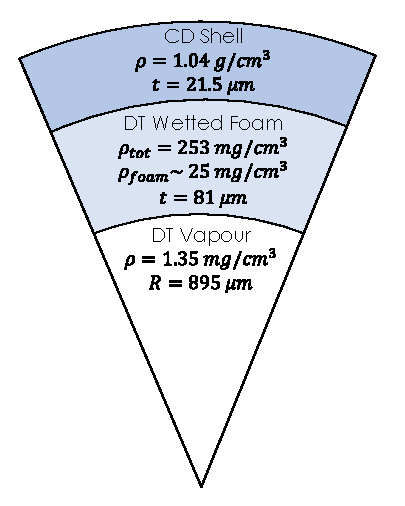
\includegraphics[width=.35\textwidth]{figures/LowCR/280Capsule.pdf}}
\subfigure b){\label{fig:280Hydro}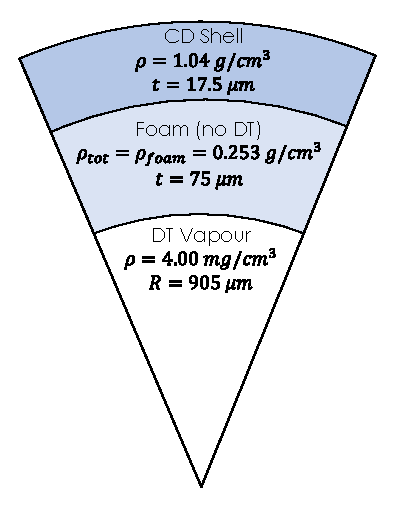
\includegraphics[width=.35\textwidth]{figures/LowCR/280Hydro.pdf}}
\caption{\label{fig:Hydroequivalent} a) The original 280 kJ wetted foam capsule. b) The 280 kJ hydroequivalent capsule. A higher foam density is used to compensate for the lack of DT, to give an equivalent layer density. The optimisation process if then reran, resulting in slightly different laser timings and layer thicknesses.}
\end{figure}

Hydro-equivalent versions of three different implosions have been developed, and are displayed (and compared to the original designs on which they are based) in Table \ref{tab:Hydroequivalent}. In each case, the new capsule was optimised according to the same optimisation procedure used in the previous chapter, maximising the gain of the implosion while satisfying the four criteria. In each case, this results in an implosion with much reduced yield and gain (due to the significantly reduced quantity of DT). However, the key hydrodynamic variables used to define the low instability regime - the convergence ratio, IFAR, and implosion velocity - are very similar to the original capsules, and continue to satisfy the low-instability criteria.

\begin{table}
\resizebox{\textwidth}{!}{%
\centering
\begin{tabular}{|c|c|c|c|c|c|c|}
\hline
Size multiplier &  \multicolumn{2}{c|}{0.35} & \multicolumn{2}{c|}{0.5} & \multicolumn{2}{c|}{0.65} \\ 
\hline
Hydroequivalent? & - & H.E. & - & H.E. & - & H.E.  \\
\hline
Laser energy (MJ) & 0.27 & 0.24 & 0.77 & 0.78 & 1.7 & 1.5 \\ 
Gain &  0.067 & 0.0094 & 0.19 & 0.016 & 0.75 & 0.023\\ 
Convergence ratio & 15.7 & 16.0 & 16.0 & 16.0 & 15.8 & 15.8 \\ 
IFAR & 27.5 & 28.4 & 29.7 & 29.4 & 25.1 & 29.3 \\ 
Implosion velocity (km/s) & 395.8 & 396.3 & 399.6 & 388.9 & 399.6 & 387.5\\ 
Max pulse power (TW) & 84.79 & 84.79 & 173.00 & 173.00 & 292.38 & 292.38\\ 
Pulse 2 switch on time (ns) & 2.20 & 2.70 & 2.60 & 2.50 & 3.60 & 3.70\\ 
Pulse 3 switch on time (ns) & 4.60 & 4.90 & 5.60 & 5.90 &7.80 & 7.80\\ 
Pulse 4 switch on time (ns) & 5.50 & 5.80 & 6.80 & 6.90 & 9.50 & 9.20 \\ 
Laser switch off time (ns) & 8.50 & 8.50 & 11.00 & 11.20 & 15.00 & 14.20 \\ 
Vapour/liquid boundary (\si[per-mode=symbol]{\milli\meter}) & 0.8950 & 0.9050 & 1.3050 & 1.3150 & 1.6705 & 1.7225\\ 
Liquid/CD boundary (\si[per-mode=symbol]{\milli\meter}) & 0.976 & 0.980 & 1.3950 & 1.3950 & 1.8200 & 1.8135\\ 
Outer radius (\si[per-mode=symbol]{\milli\meter}) & 0.9975 & 0.9975 & 1.4250 & 1.4250 & 1.8525 & 1.8525\\ 
Vapour density (\si[per-mode=symbol]{\milli\gram\per\centi\meter\cubed}) & 1.35 & 4.00 & 1.05 & 3.90 & 1.00 & 3.75\\
\hline
  \end{tabular}}
  \caption{Hydroequivalent implosions for three capsule size. The wetted foam implosion for each size has been included for comparison. All implosions use a four-pulse laser sequence. The hydroequivalent capsules have been optimised, resulting in slightly different values for the optimisation parameters and the laser energy, but the hydrodynamic parameters are broadly similar.}
  \label{tab:Hydroequivalent}
\end{table}

This provides a series of surrogate capsules, which could be used in room temperature experiments to validate this regime and verify the assumptions of low instability growth. These capsules could be shot, the amount of instability growth quantified, and their performance compared to the 1D simulations. If the instability growth is low and the agreement with the simulations good, then this would suggest that the four criteria used to define this regime are indeed sufficient to guarantee good agreement, and thus that the designs presented in the previous chapter would likely also perform as described in simulations. This therefore provides a route towards experimental verification of these results.

\section{Alternative laser drivers} \label{sec:AlternativeDrivers}

A possible way to increase fusion performance is to increase the frequency of the laser driver. Higher frequency lasers have have a higher energy coupling with the plasma, which results in a greater ablation pressure for equivalent laser intensity. The higher frequency also has a higher critical density and can thus propagate further into the plasma, leading to increased laser absorption (since the light travels through more material) and a higher density blow-off \cite{Obenschain2020}. The lower laser wavelength also means that higher intensities are permitted before the onset of significant parametric instability growth \cite{Montgomery2016} (as highlighted by the $I \cdot \lambda^2$ criteria for the low-instability regime). 

The simulation platform described in the previous section is well-suited to an investigation of different laser drivers. The laser frequency can easily be changed in HYADES, and the same style of optimisation campaign can then be performed. The purpose of doing such is two-fold: the possible performance in the low-instability regime is further investigated, and the possible impact of increasing the laser driver can be investigated, quantified, and compared to the third-harmonic simulations in the previous section (all in a regime where reasonable agreement is expected between experiment and simulation). Two different laser drivers are considered in this section: a 193 \unit{\nano\meter} laser with a similar pulse profile to the previous simulations, and a novel `two-colour' laser pulse scheme.

\subsection{Background to possible IFE laser drivers}

Designs for IFE power plants have a number of requirements, including high laser efficiency, broadband laser operation, and (obviously) high gain. There are two main laser technologies that are seen as potentially satisfying these requirements; diode-pumped solid-state lasers (DPSSL) and electron-beam pumped excimer lasers, such as KrF or ArF \cite{Craxton2015}. 

The DPPSL fundamental wavelength is 1.05 \unit{\micro\meter}, which can be frequency tripled to 0.35 \unit{\micro\meter} - the same frequency used at the NIF, and that the previous simulations were performed for. The DPSSL technology is similar to that used at the NIF, where flash lamps are used to pump a solid state glass gain medium; but for DPSSL, the flashlights (which are inefficient, as they emit broadband light) are replaced with diode lasers which pump the medium at the appropriate frequency much more efficiently\footnote{The gain medium is not necessarily the same Nd:glass medium currently used at the NIF, but this is an option under consideration}. 

Excimer lasers are naturally higher frequency, with fundamental wavelengths of 0.258 \unit{\micro\meter} for KrF lasers and 0.193 \unit{\micro\meter} for ArF lasers. In excimer lasers, the gain medium is a gaseous mixture of a noble gas (Kr or Ar) and a halide (F). An electrical discharge is driven through the medium to excite it, leading to the formation of exciplex molecules - these emit UV radiation when they relax, and it is this relaxation which is used to provide the laser emission. There have been a number of excimer lasers developed (including Sprite/Titania at the CLF \cite{Divall1996}, Garpun at Lebedev Physical Institute \cite{Zvorykin2006}, and Nike at the NRL \cite{Obenschain1996}), but these have so far been limited to energies below 10 kJ. 

The `high average power laser' programme conducted between LANL and NRL investigated future laser drivers for IFE power-plants, and led to the development of high repetition rate lasers based on the two technologies \cite{Craxton2015}; the Electra KrF laser at the NRL (which could produce energies of up to 700 J and repetition rates of up to 5 Hz), and the Mercury DPSSL laser an LANL (which gave shots greater than 50J, with a repetition rate of up to 10 Hz \cite{Sethian2010}. Both lasers performed well, and this led to the conclusion that either technology could be viable for an IFE power plant and development of both approaches should be pursued.

Both approaches have their advantages. DPSSL lasers are likely more robust (as they are entirely solid-state), and the lower fundamental frequency is beneficial for preventing damage to laser optics \cite{Sethian2010}. However, excimer lasers have some strong advantages for direct-drive fusion performance. This includes the higher frequency (and thus greater laser absorption), but also a very smooth beam profile (desirable for direct-drive), good capability for focal zooming, and an inherently high bandwidth (significant for preventing parametric instability growth). These properties mean that simulations suggest that KrF or ArF lasers could be used to achieve higher gains for equivalent energies than DPSSL lasers. There is therefore a continuing interest in these technologies, as demonstrated by recently published simulations suggesting significant gains at low energies using ArF lasers for shock ignition \cite{Obenschain2020}.

\subsection{ArF lasers}

Implosion optimisations were performed for a range of capsule radii, using a higher laser frequency of 193~nm. These results are therefore directly relevant to ArF lasers (for which this is the fundamental frequency), but as the changes depend only on the frequency they also indicate how moving to higher frequencies generally - be that from using a KrF laser (0.258 \unit{\micro\meter}), or using the fourth (0.263 \unit{\micro\meter}) or fifth (0.210 \unit{\micro\meter}) harmonic of Nd:glass - would influence performance. In the low instability-regime outlined in the previous chapter, the maximum permitted laser power is set by a limit on $I \cdot \lambda^2$; increasing the frequency thus meant that the laser power could also be increased, while continuing to satisfy this criteria. All the laser powers were thus scaled accordingly. The pulse profile, capsule design, and simulation settings were otherwise unchanged from the previous simulations.

Three different capsule sizes were simulated and optimised by two summer students (Heath Martin and Rusko Ruskov) under my supervision. I provided the code required to do the simulation campaign, adjusted this to provide simulations at the new frequency with the new pulse powers, and then trained and supervised the two students as they performed the optimisation. The tabulated results are displayed in \ref{tab:TwoColourTable}, and are plotted in \ref{fig:ArF and Two colour}.

\begin{figure}[ht]
\centering
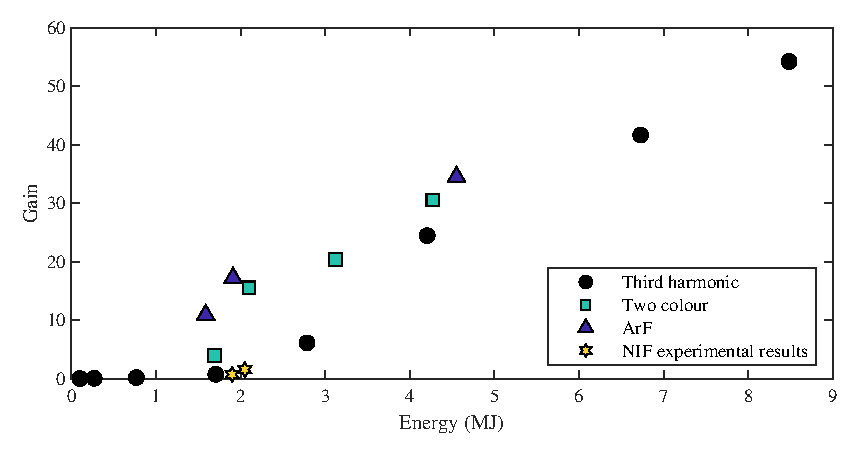
\includegraphics{figures/FurtherSims/ArFandTwoColour.eps}
\caption{A plot of the gain vs the laser energy for simulations using the three different laser drivers. The NIF 210808 experimental shot, and the recent NIF ignition shot, have been included for comparison.}
\label{fig:ArF and Two colour}
\end{figure}

\begin{table}
\resizebox{\textwidth}{!}{%
\centering
\begin{tabular}{|c|c|c|c|c|c|c|c|}
\hline
Laser driver   & \multicolumn{3}{c|}{ArF} & \multicolumn{4}{c|}{Two-colour} \\ 
\hline
Size multiplier & 0.45 & 0.5 & 0.65 & 0.5 & 0.65 & 0.75 & 0.85 \\
\hline
Total laser energy (MJ)  & 1.59 & 1.91 & 4.55 & 1.69 & 2.10 & 3.12 & 4.27\\ 
3rd harmonic energy (MJ) & - & - & - & 0.92 & 1.82 & 2.75 & 3.96 \\
ArF energy (MJ)  & 1.59 & 1.91 & 4.55 & 0.77 & 0.28 & 0.37 & 0.32\\
Gain & 10.9 & 17.3 & 34.5 & 4.0 & 15.5 & 20.4 & 30.5 \\ 
Convergence ratio  & 16.0 & 15.9 & 14.0 & 16.0 & 16.0 & 16.0 & 16.0\\ 
IFAR  & 11.3 & 10.5 & 8.5 & 16.1 & 20.4 & 23.8 & 23.4 \\ 
Implosion velocity (km/s)  & 390.7 & 398.9 & 360 & 391.1 & 399.9 & 396.4 & 391.6\\ 
Max 3rd harmonic power (TW)  & - & - & - & 173 & 292 & 389 & 500\\
Max ArF laser power (TW)  & 464 & 572 & 967 & 274 & 463 & 617 & 792\\ 
Pulse 2 switch on time (ns)  & 3.90 & 3.50 & 2.50 & 1.95 & 3.00 & 2.70 & 3.50\\ 
Pulse 3 switch on time (ns)  & 7.10 & 7.50 & 8.90 & 4.35 & 7.80 & 7.20 & 9.10\\ 
Pulse 4 switch on time (ns)  & 8.85 & 9.25 & 10.80 & 8.05 & 9.40 & 9.10 & 11.10\\ 
2nd laser switch on time (ns)& - & - & -  & 10.00 & 14.70 & 15.20 & 18.20 \\
Laser switch off time (ns)  & 11.95 & 12.25 & 15.10 & 12.80 & 15.30 & 15.80 & 18.60\\ 
Vapour/ice boundary (\si[per-mode=symbol]{\milli\meter})  & 1.072 & 1.210 & 1.435 & 1.230 & 1.645 & 1.933 & 2.210\\ 
Ice/CD boundary (\si[per-mode=symbol]{\milli\meter})  & 1.200 & 1.340 & 1.780 & 1.360 & 1.818 & 2.100 & 2.374\\ 
Outer radius (\si[per-mode=symbol]{\milli\meter}) & 1.2800 & 1.425 & 1.8525 & 1.425 & 1.8525 & 2.1375 & 2.4225 \\ 
Vapour density (\si[per-mode=symbol]{\milli\gram\per\centi\meter\cubed})& 1.00 & 1.03 & 0.60  & 1.02 & 1.05 & 1.00 & 1.01 \\
\hline
  \end{tabular}}
  \caption{Simulation parameters for the two-colour and high frequency implosions.}
  \label{tab:TwoColourTable}
\end{table}

It can be seen in Figure \ref{fig:ArF and Two colour} that the ArF implosions display a significant improvement in gain for a given energy compared to the previous third-harmonic simulations. A gain of 11 can be achieved for around 1.6 MJ of laser energy, which is an order of magnitude higher than was predicted previously. This clearly displays the potential benefits of using a higher frequency laser driver. It should again be noted that this is in the low-instability regime, and thus it should be expected that instability growth would be minimal and 1D simulations should give a reasonable estimate of performance.

It is worth commenting on the physical properties of these implosions. The higher laser power but comparable implosion velocity when using ArF lasers means that under this optimisation procedure, for a given capsule radius the ArF laser energy used is much higher than that used for the third-harmonic. Alternatively, this means that for an equivalent energy ArF and third-harmonic laser energy, the ArF implosion will feature a smaller capsule radius. The use of the higher frequency essentially shifts the ignition curve (the relationship between gain and energy) to lower energies, meaning that break-even, ignition, and a particular gain all require lower energies to achieve.

\subsection{Two-colour implosions}

Higher frequency lasers (whether excimer or higher harmonics of Nd:glass) are less technologically developed than third-harmonic Nd:glass lasers, and have not yet been demonstrated at such high energies. This makes the previous ArF results challenging to achieve in practice. As such, an alternative driver-scheme is proposed, where the higher frequency laser is used to supplement a third-harmonic driven implosion. This is a compromise solution, which allows some of the performance benefits from using high frequency lasers to be achieved, while reducing the energy demanded from these novel laser technologies. The high-frequency energies required are still greater than are currently available, but are far more achievable than those in the previous section. This concept will be referred to as a `two-colour' approach.

The laser scheme proposed is shown in figure \ref{fig:Two colour sequence}. A four-pulse third-harmonic sequence is applied, with the same pulse-profile as used in the previous simulation campaigns. Then, at a late stage in the implosion, a high-power short-duration pulse is applied at the higher ArF laser-frequency. While the four-pulse sequence was already at the maximum allowed power under the $I \cdot \lambda^2$ criteria, the lower wavelength of the final pulse means a higher power can be tolerated. The $I \cdot \lambda^2$ criteria is applied separately for the two lasers, given the large separation in wavelength between them (it has been demonstrated previously that using multiple frequencies leads to lower instability growth \cite{Follett2018}).

\begin{figure}[ht]
\centering
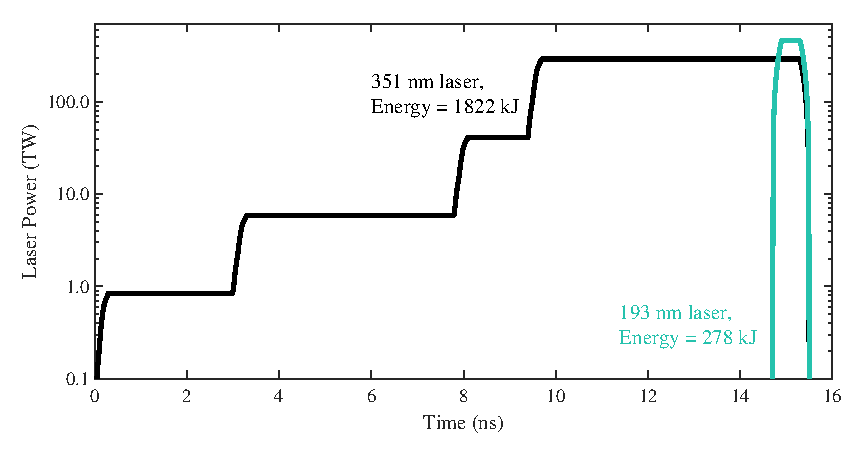
\includegraphics{figures/FurtherSims/TwoColourLaser.eps}
\caption{A log plot of laser power vs time for the 0.65 size two-colour implosion (which achieves a gain of 15.5). A four-pulse third harmonic laser is applied, which is supplemented by a single late pulse from an ArF laser. The ArF has a higher frequency, and thus a higher peak power can be used than for the third harmonic laser.}
\label{fig:Two colour sequence}
\end{figure}

As before, the four criteria for the low-instability regime continued to be applied. In particular, this meant that the implosion velocity was still unable to increase past 400 \unit{\kilo\meter\per\second} at any point in the implosion. This meant that heavier (thicker) shells were used which were accelerated to lower velocities by the third-harmonic laser, so that they continued to remain under the 400 \unit{\kilo\meter\per\second} limit once the high-frequency pulse has been applied. The addition of a late pulse made the optimisation more challenging, as it added an additional optimisation parameter (the switch on time of the final pulse). A lower maximum ArF laser power was used for the late pulse than the maximum permitted under the $I \cdot \lambda^2$ constraint, or than was used for the ArF-frequency implosions; this appeared to be beneficial in preliminary simulations, but the more challenging optimisation procedure meant this parameter was not investigated further. After I wrote the code to implement these changes and performed some initial simulations, the optimisations were again performed by Heath Martin and Rusko Ruskov under my supervision. The results are displayed alongside those of the ArF simulations in Table \ref{tab:TwoColourTable} and Figure \ref{fig:ArF and Two colour}.

It can be seen that, as expected, the results for the two-colour implosions consistently fit somewhere between those of the third-harmonic and ArF-frequency results. At 1.7 MJ, the two-colour sequence results in a gain of 4; lower than the gain of 11 achieved for a 1.6 MJ ArF sequence, but a significant improvement compared to the gain of 0.8 achieved using third-harmonic driver. Perhaps more significant is the gain of 15.5 achieved at 2.1 MJ, requiring only 280 kJ of the high-frequency laser. While still a significant increase over current energies for these lasers, this provides a clear demonstration of how this technique leads to significant increases in gain for much more moderate amounts of high-frequency laser energy; although it should be noted that this scheme would require a facility where the capsule can be irradiated uniformly using two different frequencies at the same time\footnote{This approach would therefore perhaps be more suited to higher harmonics of Nd:glass rather than an ArF laser, as then a single laser system could be used with the higher frequency provided by further frequency conversion on some of the beams}.

There are other features of these implosions that it is interesting to comment on. First, note the variation in the proportion of the total energy within the late pulse. This is likely a result of the difficulty in optimising these sequences, due to the additional optimisation parameter. While these simulations are indicative of the levels that may be obtained, it thus appears that further optimisation may be possible. The low IFAR values of these implosions should also be noted, highlighting that this increased performance is achieved by accelerating thicker shells compared to the third-harmonic implosion. Some caution is required here when predicting the amount of Rayleigh-Taylor growth based on these IFAR values, due to the fact that the IFAR quoted corresponds to that measured when the capsule shell is at two thirds of the initial capsule radius. This is before the late-pulse is applied, and thus the IFAR value contains no information about the effect of this late pulse. Trends between the IFAR value and the amount of instability growth are based on experiments and theory which do not include the impact of this late pulse, and thus do not necessarily apply in the same way to the two-colour approach. However, low-instability growth is still predicted, due to three reasons: 1) the IFAR values are low even compared to the criteria of 30, allowing for some further compression of the shell; 2) the three additional criteria also serve to minimise instability growth; and 3) as the additional pulse is applied late, there is less time for any instabilities that it potentially seeds to grow. If this approach were to be pursued, these predictions should be tested with two-dimensional simulations.

\subsection{The burning plasma parameter for alternative laser drivers}

The burning plasma parameter for all of the implosions shown in Figure \ref{fig:ArF and Two colour} has been calculated\footnote{The terms were evaluated as follows: 1) the total work done $E^\mathrm{{tot}}_{\mathrm{PdV}}$ was evaluated as the sum of hotspot and shell kinetic and thermal energies, at the point during the deceleration of the shell where these two energies are equal. This corresponds to a period where the total energy of the capsule is constant, just prior to the onset of fusion reactions. 2) the deposited alpha energy over the full capsule was used rather than the hotspot for $E_\mathrm{\alpha}$, assuming that this absorption is dominated by the hotspot \cite{Christopherson2018}. These quantities were evaluated in this way to reduce the dependence of the calculated quantity on the exact position of the hotspot interface, so that it was more robust to issues with hotspot tracking.}, using Equation \ref{eqn:Qtot defn}. The ArF and two-colour implosions can all be seen to be well within the burning-plasma regime, with burning plasma parameters of around 10 and above. It can be seen that the 1.7 MJ third-harmonic implosion is the first third-harmonic result to achieve burning plasma.

\begin{figure}[ht]
\centering
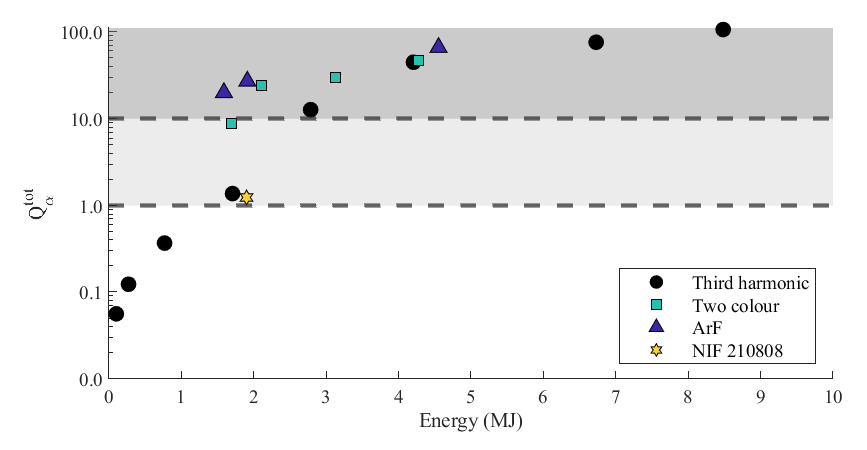
\includegraphics{figures/FurtherSims/QTwoColour.eps}
\caption{A log plot of the total capsule burning plasma parameter $Q^\mathrm{{tot}}_{\mathrm{\alpha}}$ vs laser energy for the optimised capsules using the three laser drivers. Values of $Q^\mathrm{{tot}}_{\mathrm{\alpha}} = 1$ and $Q^\mathrm{{tot}}_{\mathrm{\alpha}} = 10$ are indicated.}
\label{fig:TwoColourQ}
\end{figure}

NIF shot data for N210808 (the 1.3 MJ yield shot \cite{Abu-Shawareb2022}) has also been estimated and plotted on this graph, but this is very approximate and illustrative only\footnote{To do this, the `hotspot burning plasma parameter' for N210808 was estimated from the figure in \cite{Abu-Shawareb2022}. The hotspot compression energy is typically around roughly half that of the total compression energy \cite{Betti2015}, and so the `total capsule burning plasma parameter' plotted here is likewise assumed to be half that of the reported hotspot burning plasma parameter.}. The burning plasma parameter suggests that the performance of this shot was comparable to the simulated performance of the third-harmonic low-instability targets (as was likewise observed when comparing the gain of these implosions). Insufficient data was available at the time of writing to plot this for the recent 3.5 MJ yield shot. 

\subsection{The zoomed focus technique}

Another potential benefit of these approaches are their compatibility with the `zoomed focus' technique. As the implosion occurs and the capsule is compressed, the critical density surface will move inwards from the initial capsule radius. However, the laser focus normally remains fixed at this original position. This smaller radius means that some light that previously would encounter the critical density surface will now miss it entirely. This results in reduced laser absorption. In addition, an increased amount of light travelling through the coronal plasma will contribute to increased cross-beam energy transfer, resulting in further decreased absorption and less uniform compression.

The `zoomed focus' or `zooming focus' technique requires changing the focus of the laser during the course of the implosion, allowing it to be better matched to this reduced critical density surface \cite{Kehne2013, Eimerl2014}. This is feasible but complex to achieve using conventional Nd:glass lasers \cite{Obenschain2015}, but is reasonably straight-forward to implement on excimer lasers  (due to differences in how the laser is smoothed) and has been successfully demonstrated on the (KrF) Nike laser \cite{Kehne2013}. This technique leads to reduced laser losses, and thus improvements to the fusion performance. The two-colour scheme is also a natural fit for such a technique; the high frequency laser can have a smaller focal spot than the third-harmonic laser, providing the `zoom' late in the implosion.

This effect is not included in the simulations presented here. In the 1D HYADES simulations, the laser provides perfect uniform and spherical illumination, and the laser is focused at the centre of the target \footnote{It is possible in HYADES to use ray-tracing to simulate the impact of rays of light travelling at non-normal angles. However, it is not possible to include the effect of the finite spot-size, rather than an infinitesimally small focus. This is not sufficient to simulate the effect described here.} - meaning that the negative effects discussed above are not included. These simulations represent an ideal case, while the zoomed focus technique is an attempt to solve a non-ideal and practical problem. It should therefore be expected that implementing focal zooming (as could be done on ArF or two-colour implosions) would reduce a degradation mechanism not seen in the code, and thus give performance closer to that simulated than would be achieved without using this technique.

\section{Auxiliary heating using relativistic electron beams} \label{sec:AuxiliaryHeating}

In Chapter \ref{ch-lowCR}, it was noted that the areal density of the hotspot for the 0.8 MJ capsule exceeded 0.3 \unit{\gram\per\centi\meter\cubed}. This is significant, as this is the areal density generally considered to be required for ignition to occur. If the ion temperature could be increased in some way, it may be possible for this capsule to ignite and thus the gain to be significantly increased.

In this section, an auxiliary heating scheme is investigated which could potentially provide this increase in ion temperature. This is based on the scheme proposed and described by Ratan \textit{et al.} \cite{Ratan2017}. A brief description of the scheme will be provided, summarising how it was understood at the time that this work was performed. Then, how this was applied to the simulations from Chapter \ref{ch-lowCR} will be described, before the results are discussed. This scheme will then be applied to some of the higher-gain alternative driver simulations, along with new capsules optimised for areal density (rather than yield). Finally, more recent work (not performed by the author) with implications for how this scheme would be applied in practice are briefly discussed.

\subsection{Principles of the auxiliary heating scheme}

The scheme as described by Ratan \textit{et al.} \cite{Ratan2017} works as follows. Two relativistic electron beams are produced and fired at a central hotspot implosion, such that they overlap within the hotspot. This is most compatible with low convergence ratio implosions, which have a large hotspot in which these beams can be overlapped. The electron beams lead to a bump-on-tail instability which results in the growth of Langmuir waves, with energy transferred from the electron beam to these waves. These waves eventually undergo Landau damping, which smooths the distribution function and results in the transfer of the energy within these waves to the bulk electrons in the plasma; this leads to an increase in the electron temperature within the hotspot. Ion-electron collisions lead to an equilibration of the electron and ion temperatures, and so the ion temperature also increases. This process takes place over the order of a few picoseconds, which is very fast compared to the compression timescales of the capsule. In their investigation of this heating scheme, Ratan \textit{et al.} performed Vlasov simulations of this heating mechanism for fusion relevant conditions, and found that energy was transferred from the electron beams to the electrons in the hotspot with an efficiency of 18 \%.

How the electron beams are generated is not the focus of this work, but is a topic that has been explored elsewhere due to the application of such beams to fast ignition \cite{Tabak2005, Kemp2014}. Typically, it is expected that an ultra-high intensity short pulse laser would generate the electrons in the plasma through a range of potential interactions. These can include SRS and TPD in the low-density region of the plasma,  resonant absorption, vacuum heating\footnote{Also referred to as `Brunel' or `Not-so-resonant resonant absorption', this is a case of resonant absorption where electrons within the skin-depth of the critical density plasma are dragged out by the (rapidly-decaying) electric field associated with the EM wave, and then accelerated back into the high density region at high velocity a half-cycle later}, and $\vec{j} \times \vec{B}$ heating\footnote{This effect is important for high intensities, where the magnetic component of the EM wave cannot be neglected. If the wave travels normal to the critical density surface and the electric field causes electrons to oscillate in the direction of the E field, then the $\vec{v} \times \vec{B}$ component of the Lorentz force will also be normal to the surface, and electrons can be accelerated across the critical density surface}\cite{Wilks1997}.

The auxiliary heating scheme appears well suited to the designs presented in the previous chapter. It would be expected to drive a rapid increase in the ion temperature (as is required), leading to an increase in the fusion yield. The low-convergence ratio nature of these implosions also provide a large hotspot for the overlap of the electron beams. Since the work in this section was performed, further research into this scheme has improved and changed the understanding of how such a scheme would operate \cite{Lee2023}; these new developments are discussed in Section \ref{sec:AuxHeatingDevlopments}.

\subsection{Simulating auxiliary heating in Hyades}

Simulating auxiliary heating of these implosions is challenging, due to the multi-scale nature of such a setup. Fluid codes such as HYADES can simulate the implosion, but cannot simulate the auxiliary heating scheme as they do not include the necessary physics (it is not possible to generate Lagnmuir waves or to simulate Landau damping in such a code). Alternatively, particle-in-cell or Vlasov codes do include these effects, but cannot be feasibly ran over the large time and spatial scales required to simulate the implosion. As such, approximations must be made.

In this work, HYADES is used to estimate the impact of the auxiliary heating, by estimating the effect that such a scheme would have on the electron energy. The Vlasov simulations performed by Ratan \textit{et al.} suggest that, for relevant conditions, the heating scheme would lead to an increase in the bulk plasma electron energy in the centre of the capsule. As such, HYADES simulations were performed where some amount of electron energy was added to the central zones (for convenience, this was done over those zones which initially contained the DT vapour at the start of the implosion), over a 7 picosecond window (corresponding to the timings from \cite{Ratan2017}) at a point just before the bang time of the implosion. The electron beams, Langmuir waves, and Landau damping are not simulated - but the estimated impact of such a scheme is. The effect this heating has on the fusion performance of the implosion can thus be investigated.

Figure \ref{fig:EnergyDist} shows the kinetic, thermal, and total energy in the hotspot for two HYADES simulations, in a 0.4ns window around the bang-time. Figure \ref{fig:EnergyDist} (a) considers an implosion without auxiliary heating. As the shell decelerates and the capsule stagnates, the kinetic energy decreases and the thermal energy increases accordingly. The total energy is initially constant, but a small amount of fusion reactions occur which leads to a small increase in energy (through alpha self-heating). Figure \ref{fig:EnergyDist} (b) displays the same implosion, but where 20 kJ of electron energy is added in order to simulate the effect of auxiliary heating. This leads to a rapid increase in the thermal energy. This then leads to a significant increase in the amount of fusion reactions, as shown by the much greater subsequent increase in total energy. It can also be seen that the increase in energy from the alpha self-heating is larger than that used for the auxiliary heating.

\begin{figure}[ht]
\centering
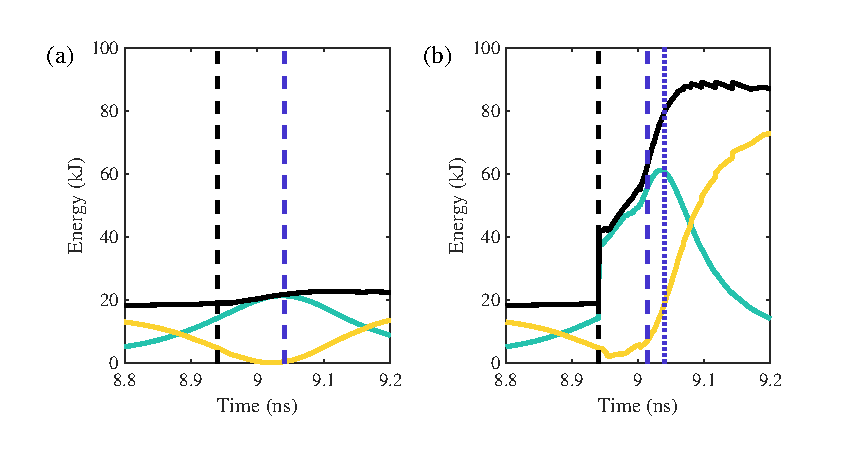
\includegraphics{figures/FurtherSims/EnergyDist.eps}
\caption{Plots showing the total (black), thermal (teal) and kinetic (yellow) energy in the hotspot of the same implosion both with (a) and without (b) 20 kJ of energy added to the electrons. The dashed black line in both plots displays the time at which the energy should be added to achieve the maximum increase in yield. The bang-time for each implosion is displayed by a dashed blue line. For the heated implosion, the bang-time from (a) is indicated by a dotted line; it is clear that applying heating means the bang-time occurs at an earlier time.}
\label{fig:EnergyDist}
\end{figure}

This demonstrates that adding electron energy in this way can indeed be used to improve the fusion performance of the capsule. In the following sections, this approach is applied to and investigated using four of the capsules developed in Chapter \ref{ch-lowCR}. The key data for these capsules has been summarised in Table \ref{tab:Heating capsules} for convenience, where they are labelled as capsules A-D. In the simulations discussed in this section, the implosion is unchanged from that reported in Table \ref{tab:ThirdHarmonic} apart from the addition of the electron energy. The capsule and laser parameters are not varied. The laser in the simulation - the four-pulse third-harmonic profile optimised in the previous chapter - will be referred to as the `long-pulse' laser energy, to differentiate it from the hypothetical `short-pulse' laser that would be used to generate the electron beam. The phrase `heating energy' will be used to describe the added electron energy; this is varied independently of the long-pulse laser, which always has the energy described in Table \ref{tab:ThirdHarmonic}.

\begin{table}
\centering
\begin{tabular}{|c|c|c|c|c|}
\hline
Capsule label &  A & B & C & D \\ 
\hline
Size multiplier & 0.25 & 0.35 & 05 & 0.65 \\
`Long-pulse' laser energy (kJ) & 101  & 270 & 768 & 1710 \\ 
Gain & 0.030 & 0.067 & 0.19 & 0.75\\ 
\hline
  \end{tabular}
  \caption{The four capsules (labelled A-D) for which the auxilliary heating is applied to. Only the key parameters are shown; refer to Table \ref{tab:ThirdHarmonic} for full simulation details}
  \label{tab:Heating capsules}
\end{table}

\subsection{Timing of electron energy deposition}

The timing at which the heating is applied to the implosion has a large impact on the increase in fusion performance. To investigate this, simulations were performed where 4 kJ of electron energy was added at different times around the bang-time of the unheated implosions. The results are displayed in Figure \ref{fig:HeatingTiming}. The metric used here to evaluate performance is the relative yield amplitude, which is defined in this paper as the yield of the capsule when the heating is applied, compared to the yield of the capsule when no electron energy is added \footnote{Note that this is different to it's conventional usage comparing the yield when alpha self-heating is/isn't included.}.

There is a clear peak in the yield amplification as a function of time for each capsule, indicating the optimal time for the heating to be applied. This optimal time is also that displayed in Figure \ref{fig:EnergyDist}, where it can be seen that it occurs just before the minimum in kinetic energy (as the shell stops moving inwards), and just before significant amounts of fusion reactions begin. This is unsurprising: adding the energy to the hotspot prior to this point would make it harder to compress and thus reduce the density, while adding it after significant fusion has occurred will mean that the burn wave has already started to propagate, and will mean that the added energy is smaller relative to the energy of the system. The same behaviour and optimal timings were found when the simulations were repeated using 20 kJ of injected energy, suggesting these optimal values are independent of the amount of energy added.

\begin{figure}[ht]
\centering
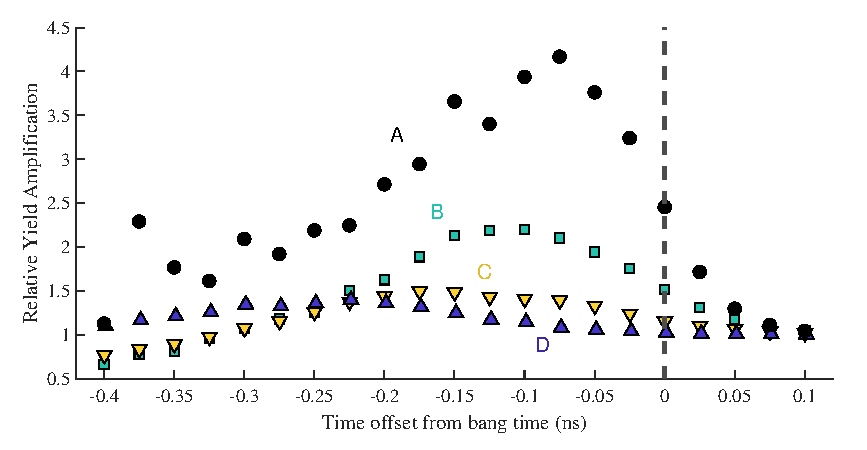
\includegraphics{figures/FurtherSims/HeatingTiming.eps}
\caption{Relative yield amplification for the capsules A-D as a function of time at which 4 kJ of electron energy is added. The capsule labels correspond to those in Table \ref{tab:Heating capsules}. The increased variation in capsule A compared to the others is likely due to the low gain of that capsule, as small changes in performance thus have a larger relative effect.}
\label{fig:HeatingTiming}
\end{figure}

\subsection{Magnitude of deposited electron energy}

Further simulations then investigated how the fusion performance with the amount of electron energy added. Between 3 to 60 kJ of electron energy was deposited for each of the four implosions, with the energy injected at the optimal time for each implosion identified from Figure \ref{fig:HeatingTiming}. The results are displayed in Figure \ref{fig:HeatingPower}. It can be seen that (as expected) adding more energy has a larger impact on the yield amplification, and even modest amounts of injected energy can have a significant effect. The relative yield amplification decreases as the capsule size increases; this is as expected, since 1) the larger capsules are higher energy, and thus the deposited electron energy is a smaller proportion of the capsule energy, and 2) the yield of the unheated capsule will be higher, and so a larger increase in yield is required for the same relative amplification.

\begin{figure}[ht]
\centering
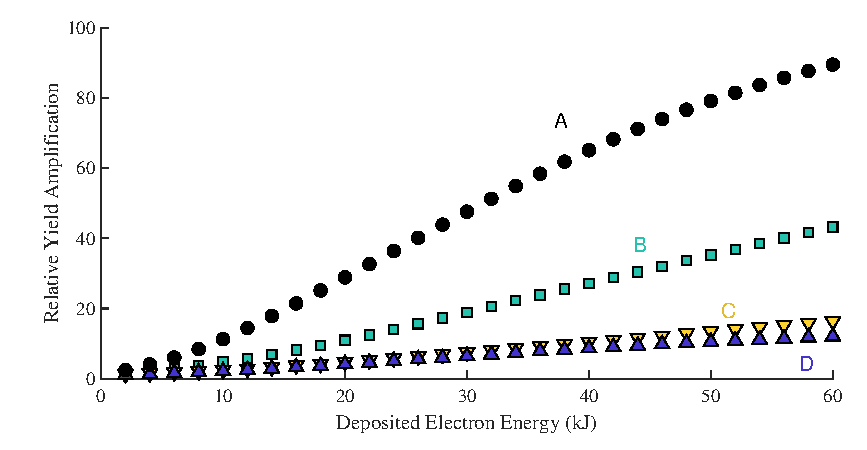
\includegraphics{figures/FurtherSims/HeatingPower.eps}
\caption{Relative yield amplification for capsules A-D as a function of the amount of deposited electron energy. The energy is injected at the optimal time for each capsule identified from Figure \ref{fig:HeatingTiming}.}
\label{fig:HeatingPower}
\end{figure}

The relative yield increase is largest for the smallest capsule (A), where 10 kJ of deposited energy gave over 10 times yield amplification, and 60 kJ amplified the yield by a factor greater than 80. Even for the largest capsule (D), 10 kJ of deposited energy is sufficient to double the yield, while 60 kJ amplifies the yield by over 12 times. This clearly demonstrates the potential this scheme has for increasing capsule performance.

\subsection{The burning plasma parameter for heated capsules}

The (total capsule) burning plasma parameter $Q^\mathrm{{tot}}_{\mathrm{\alpha}}$ has been evaluated for the heated capsules A-D, and is displayed in Figure \ref{fig:HeatedQ}
as a function of the deposited energy \footnote{The terms were evaluated as follows: 1) the total work done $E^\mathrm{{tot}}_{\mathrm{PdV}}$ was evaluated as the sum of hotspot and shell kinetic and thermal energies just after the electron energy was added, such that the deposited energy is included in the calculation 2) the deposited alpha energy over the full capsule was used rather than the hotspot for $E_\mathrm{\alpha}$, assuming that this absorbtion is dominated by the hotspot \cite{Christopherson2018}}. These results again show the improvement in performance for all four implosions when auxiliary heating is applied. While capsule D is already within the burning plasma regime, it can be seen that auxiliary heating also enables capsules B and C to enter this regime. When the largest amounts of heating are added capsule D sees an increase in the burning-plasma parameter of almost a full order of magnitude, approaching $Q^\mathrm{{tot}}_{\mathrm{\alpha}} = 10$. This indicates that self-heating adds almost ten times more energy to the hotspot that is added through external compression, suggesting a very well-performing implosion.

\begin{figure}[ht]
\centering
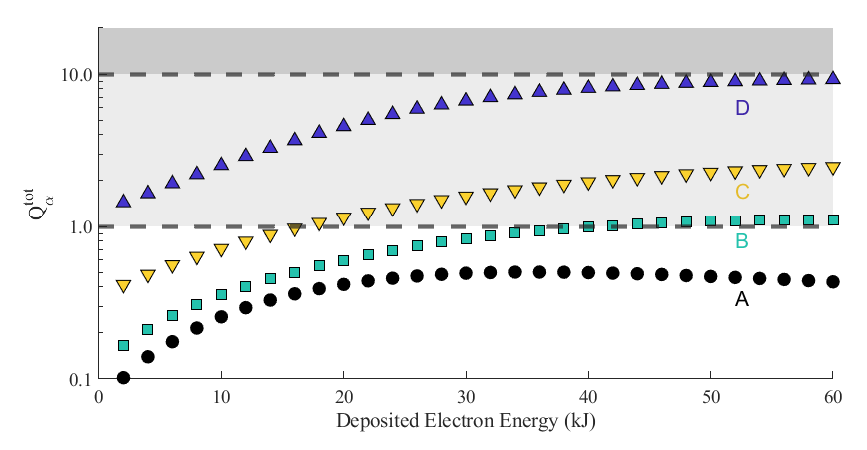
\includegraphics{figures/FurtherSims/QHeatingPlot.eps}
\caption{A log plot of the total capsule burning plasma parameter $Q^\mathrm{{tot}}_{\mathrm{\alpha}}$ vs deposited electron energy for the four capsules. Values of $Q^\mathrm{{tot}}_{\mathrm{\alpha}} = 1$ and $Q^\mathrm{{tot}}_{\mathrm{\alpha}} = 10$ are indicated.}
\label{fig:HeatedQ}
\end{figure}

\subsection{Estimating the gain of heated capsules}

Despite the challenges in calculating gain for these capsules, it is still the ultimate metric of interest for inertial fusion energy applications. The gain has therefore been estimated using values for the relevant efficiencies from the literature. These efficiencies are not known to high accuracy, and thus the gains presented in this section are indicative only. There are two processes involved for which efficiencies must be estimated: 1) the deposition of energy into the plasma via the electron beams; and 2) the generation of the electron beams via short-pulse laser. The first of these conversion efficiencies can be taken from the Vlasov-Maxwell simulations reported by Ratan \textit{et al.} \cite{Ratan2017}, which found that the electron beams deposit electron energy into the hotspot with an efficiency of 18 \%.

Previous research on fast ignition has investigated electron-beam generation using short-pulse lasers, and have produced a range of estimates for the efficiencies with which such beams can be generated and transported (some examples are \cite{Ma2012, Kemp2014, Kemp2009}, and the review article \cite{Norreys2014}). For the estimates used here, two results are highlighted. The first is that of \cite{Strozzi2012}, who performed particle-in-cell simulations for an ignition scale plasma; they estimated an overall laser to electron power conversion efficiency of 52\%, which they then coupled to a hydrodynamic code for fast ignition simulations. The second is that of \cite{Tonge2009}, who also performed particle-in-cell simulations but found that as the electron beam passes through the weakly collisional background plasma a significant proportion of the energy is lost. They therefore calculated a lower efficiency of 15\% - although they also observed that this increased with both laser power, and the time for which the laser was applied. The maximum simulation time of 2.5 ps used in their work was lower than the 7 ps that the electron energy is deposited over in the HYADES simulations, and so if this trend between deposition time and efficiency were to continue it is possible a higher efficiency could be expected.

The value of 52 \% from \cite{Strozzi2012} and 15 \% from \cite{Tonge2009} have both been used, to provide two separate estimates of the gain. Each of these efficiencies have been combined with the 18 \% simulated coupling efficiency for electron beam energy deposition into the plasma to calculate an overall efficiency for the auxiliary heating process (capturing generation of the electron beams from short pulse laser, transport of these beams, and deposition into the plasma). The short-pulse laser energies required to cause the deposited electron energies in Figure \ref{fig:HeatingPower} were thus calculated; this was added to the `long-pulse' laser energy required for each implosion to calculate the total input energy, which was then used to calculate the gain. These two sets of estimates are displayed in Figure \ref{fig:HeatedGain}.

\begin{figure}[ht]
\centering
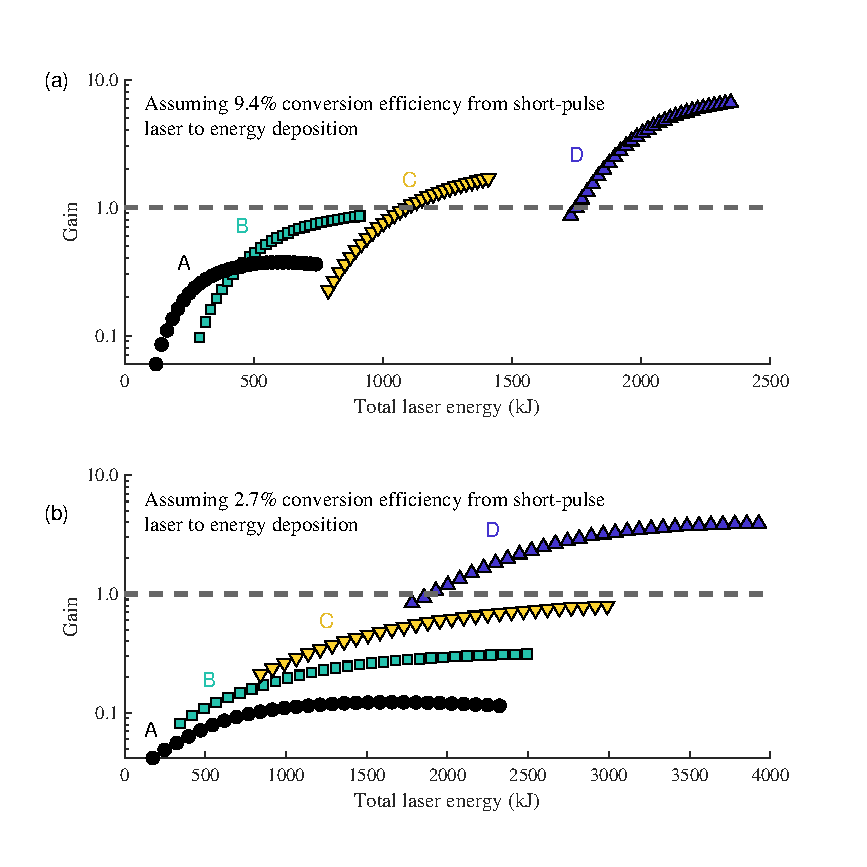
\includegraphics{figures/FurtherSims/HeatingGain.eps}
\caption{Estimated gain vs total input energy (including the `long-pulse' laser energy used to drive the implosion as reported in Table \ref{tab:Heating capsules}, and the estimated `short-pulse' laser energy required to generate the simulated amount of auxiliary heating. (a) and (b) use different estimates for the efficiency with which the heating can be generated, as indicated on the plots.}
\label{fig:HeatedGain}
\end{figure}

The general trends are the same in both figures; auxiliary heating causes an increase in gain, although this begins to saturate for larger amounts of heating energy. For the high efficiency case (a), higher gains can be achieved by using a smaller capsule with some auxiliary heating than through conventional hotspot ignition alone (as seen by the fact that lower energy capsules with a small amount of heating outperform larger capsules with no heating). This is unsurprising, as the 9.4 \% heating efficiency is higher than the roughly 6 \% efficiency for direct-drive laser compression \cite{Campbell2017, Goncharov2016}. For the lower efficiency case (b), direct-drive compression is higher efficiency, and so this is no longer observed. The saturation at large amounts of auxiliary heating is also not surprising; this is likely because both high density and high temperatures are required for high fusion yields, and at some point the density starts to become the limiting factor.

The results are obviously far more impressive for the high efficiency case, which predicts break-even for capsule C at around 1.1 MJ of total energy (using $\sim$ 350 kJ of short-pulse laser energy to deposit 32 kJ of electron energy into the hotspot), and gains of up to $\sim$ 3.5 for under 2 MJ of energy using capsule D. Given the observed trends, it appears likely that a capsule with size between B and C would achieve break-even for under 1 MJ of total energy. However, even in the low efficiency case, it is clear that auxiliary heating can still be a useful tool to improve the performance of a capsule, and capsule D can be seen to achieve break-even for under 2 MJ using this technique.

\subsection{Comparison with previous simulated and experimental results}

The results presented for capsules A-D can be compared to a range of previous results. Simulations were previously performed to estimate the impact such a scheme may have on indirectly-driven targets, which were presented in \cite{Norreys2021}. This was based on the NIF shot N160421, with a low convergence ratio and a drive energy of $\sim 800$ kJ. The greater efficiency of direct-drive implosions results in an approximately five-fold increase in the amount of energy deposited in the hotspot \cite{Campbell2017, Goncharov2016}, which means that such a capsule should be roughly equivalent to an implosion in this work with an energy of around 150 kJ. There are some minor differences between these works; the indirect-drive results demonstrate less dependence on the time at which the heating is applied, and a lower level of amplification than would be expected based on the results presented here (some differences should be expected due to the use of a different code, xRAGE, for the indirect drive simulations, and for the differences in the base implosions - with the indirect-drive implosion having significantly lower yield). Despite this the results are broadly similar between the two works, with similar trends observed in both the direct and indirect-drive simulations.

The fusion performance of capsule B is also comparable to that of NIF shots N190918, N191007, and N191110 (the capsules with record inertial fusion yields when this work was first performed \cite{Zylstra2021}), although these shots targeted higher convergence ratios over 25. These NIF shots produced neutron yields ranging from \num{0.75e16} to \num{2e16} (compared to \num{0.8e16} for capsule B without auxiliary heating) and fuel kinetic energies of $\sim$15~kJ (also similar to capsule B), for $\sim$1.9~MJ of indirect drive input energy. These shots led to predictions that laser energies of $\sim$3~MJ \cite{Zylstra2021} may have been required to achieve MJ-level yields (other predictions thought energies of up to $\sim$5~MJ may be required \cite{Zylstra2021, Cheng2021}). However, extrapolating the auxiliary heating results presented for capsule B to these implosions suggested that MJ-level yields could be achieved for a total of 2.3 MJ \footnote{This was estimated by taking the 56 kJ yield of N191110, and assuming based on implosion B in Figure \ref{fig:HeatingPower} that a yield amplification of twenty times could be achieved for 32 kJ of auxiliary heating, which would require less than 350 kJ of short-pulse laser energy assuming a conversion efficiency of 9.6 \%.}. This highlights how such a heating scheme could potentially be used to improve the performance of real NIF shots. These results could also be extrapolated for the 1.3 MJ yield shot N210808. This has a yield between those of capsules C and D; applying a similar extrapolation suggests that this yield could be doubled for only 10 kJ of deposited energy. These are illustrative examples only, but serve to demonstrate how this technique could be applicable more widely than just for the low-instability shots discussed here.

\subsection{Auxiliary heating of high gain capsules}\label{sec:auxiliary-heating-of-high-gain-capsules}
Auxiliary heating was also later applied to three of the alternative laser driver implosions. The main purpose of this was to see the effect of auxiliary heating on high gain capsules; auxiliary heating helps the capsule to achieve ignition without adding more fuel, and thus it is likely that for better performing capsules the increase in performance would be more moderate. It also allowed the combination of these technologies to be assessed. These simulations were performed by summer students Tat Li and Eugene Kim, under my supervision.

Three capsules were used: the 0.5 and 0.65 size two-colour implosions, and the 0.5 size ArF implosion \footnote{These simulations were performed a year after the capsules were first optimised, and used the updated HYADES version 01.12.05 compared to version 01.12.03 for the original simulations. Rerunning the unheated input decks using this new version resulted in a slightly increased yield. This explains why the gain at low heating levels in Figure \ref{fig:TwoColourAux} is still higher than that reported in Table \ref{tab:Heating two colour capsules}.}.  These capsules are labelled E-G in Table \ref{tab:Heating two colour capsules}. The auxiliary heating was simulated exactly as described in the previous sections, with the optimal timing for the heating identified as outlined previously, before the amount of deposited energy was varied. The results are shown in Figure \ref{fig:TwoColourAux}.

\begin{table}
\centering
\begin{tabular}{|c|c|c|c|}
\hline
Capsule label &  E & F & G  \\ 
\hline
Laser driver & \multicolumn{2}{c|}{Two-colour} & ArF \\ 
\hline
Size multiplier & 0.5 & 0.65 & 0.5 \\
\hline
`Long-pulse' laser energy (MJ) & 1.69  & 2.10 & 1.91 \\ 
Gain & 4.0 & 15.5 & 17.3 \\ 
\hline
  \end{tabular}
  \caption{The three high gain implosions (labelled E-G) for which the auxilliary heating is applied to. Full details can be found in Table \ref{tab:TwoColourTable}.}
  \label{tab:Heating two colour capsules}
\end{table}

\begin{figure}[ht]
\centering
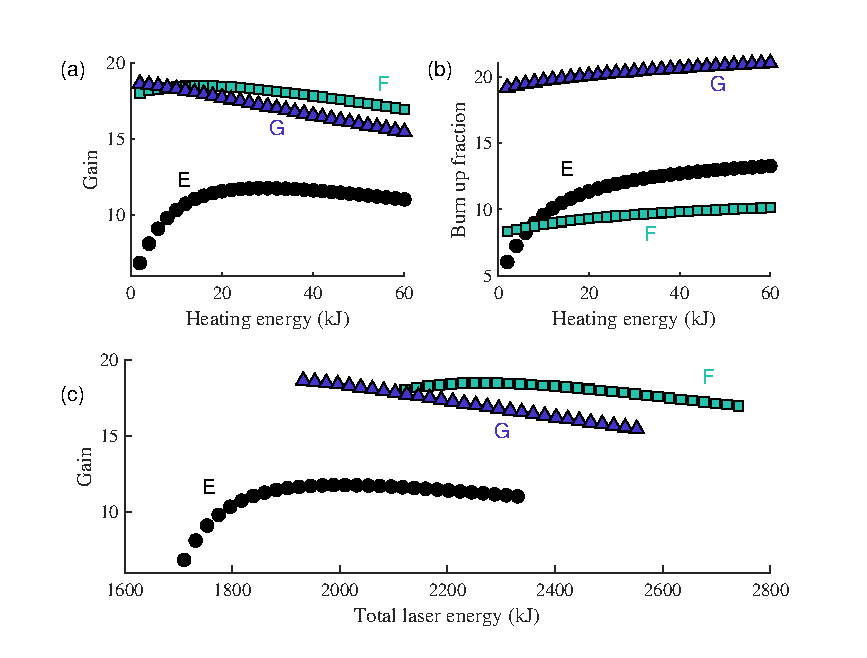
\includegraphics{figures/FurtherSims/TwoColourAux.eps}
\caption{Auxiliary heating for two two-colour implosions (E and F) and one ArF implosion (G). In (a), the estimated gain (assuming a 9.4 \% heating efficiency) is plotted as a function of the heating energy. In (b), the burn-up fraction of the three implosions versus heating energy is displayed. (c) shows the estimated gain, as a function of the total estimated input energy.}
\label{fig:TwoColourAux}
\end{figure}

As expected, it was found that for higher gain capsules, the auxiliary heating is much less beneficial. The 0.5 size two-colour implosion has the lowest base gain, and it can be seen that low amounts of added energy result moderate increases to gain, but as further heating is applied gain actually begins to decrease. This corresponds to a scenario where the additional fusion reactions generated by the increase in energy no longer compensate for the additional cost. This is not unexpected - this capsule has already achieved the conditions necessary for a large amount of fusion reactions to occur, and thus the amount of electron energy deposited (as a fraction of the hotspot energy) is much less significant than for the previous capsules.

As the yield of the unheated implosion further increases, this effect becomes even more dramatic. The 0.65 size two-colour capsule sees an even smaller fractional increase in performance, and less electron energy can be added before the gain begins to decrease. For the ArF capsule, adding electron energy offers no benefit even for low amounts of heating, and the gain decreases from the start. This is despite the unheated gain being very similar to that for the 0.65 size two-colour capsule. The reason for this is that the ArF capsule is smaller (the energy is the same due to the higher laser power), and has a much higher burn up fraction (as shown in Figure \ref{fig:TwoColourAux} (b)). The unheated ArF capsule is therefore further along it's ignition curve - it is already igniting very well, and is close to the maximum possible yield for this capsule. The two-colour capsule is larger, with more fuel and thus a higher maximum possible gain, and thus the performance can be further increased compared to the ArF capsule.

\subsection{Optimisation and heating of high areal-density capsules}
The implosions A-D (and the high gain capsules E-G) are implosions that were originally optimised for high gain, in the absence of auxiliary heating. If the auxiliary heating was included within the optimisation campaign, it may be that alternative capsule or laser pulse profiles would be found that outperform these designs.

This would add significant complexity to the optimisation, which makes it infeasible to explore without further development. However, it is possible to predict the form such an implosion may take. Auxiliary heating allows the temperature of the capsule to be significantly increased, but the areal density is unchanged. As such, it was suggested that if an implosion could be developed with a higher areal density (at the expense of a lower temperature and yield), then once auxiliary heating is applied to increase the ion temperature the resulting yield/gain may be higher than if a capsule optimised for yield was heated.

To explore this, a further two optimisations were performed. This followed the exact procedure as before, but the implosions were optimised to produce a capsule with the maximum possible areal density (i.e. the areal density of DT within both hotspot and shell), rather than yield. I again produced the changes to the code necessary to enable this, and then supervised a summer student, Tat Li, in performing the optimisations. The resulting `optimal areal density' implosions are included in Table \ref{tab:Optimal Areal Density}, along with the corresponding `high gain' version. Auxiliary heating was then applied, first identifying the optimal timing for the capsules, and then varying the deposited energy. The resulting gains (assuming the optimistic 9.4\% conversion efficiency for the heating) is then displayed in Figure \ref{fig:OptimisedRhoR}.


\begin{table}
\centering
\begin{tabular}{|c|c|c|c|c|c|c|}
\hline
Laser driver & \multicolumn{2}{c|}{Third harmonic} & \multicolumn{2}{c|}{ArF} \\ 
\hline
Size multiplier & \multicolumn{2}{c|}{0.5} & \multicolumn{2}{c|}{0.5} \\ 
\hline
Optimised for & Gain & $\rho R$ & Gain & $\rho R$  \\
\hline
Laser energy (MJ)  & 0.77 & 0.80 & 1.91 & 2.16 \\ 
Gain (original) &  0.19 & - & 17.3 & -\\ 
Gain (at time of work) &  0.19 & 0.12 & 18.7 & 24.7\\ 
Areal Density (\unit{\gram\per\centi\meter\squared}) & 0.71 & 0.76 & 1.04 & 1.30\\
Convergence ratio  & 16.0 & 15.9 & 15.9 & 15.9 \\ 
IFAR  & 29.7 & 23.2 & 10.5 & 9.0 \\ 
Implosion velocity (km/s)  & 399.6 & 358.1 & 398.9 & 361.9\\ 
Pulse 2 switch on time (ns)  & 2.60 & 3.60 & 3.50 & 4.20\\ 
Pulse 3 switch on time (ns) & 5.60 & 6.80 & 7.50 & 9.20\\ 
Pulse 4 switch on time (ns)  & 6.80 & 8.20 & 9.25 & 11.00 \\ 
Laser switch off time (ns)  & 11.00 & 12.60 & 12.25 & 14.40 \\ 
Vapour/liquid boundary (\si[per-mode=symbol]{\milli\meter})  & 1.305 & 1.290 & 1.210 & 1.150\\ 
Liquid/CD boundary (\si[per-mode=symbol]{\milli\meter})  & 1.3950 & 1.390 & 1.340 & 1.340\\ 
Outer radius (\si[per-mode=symbol]{\milli\meter})  & 1.425 & 1.425 & 1.425 & 1.425\\ 
Vapour density (\si[per-mode=symbol]{\milli\gram\per\centi\meter\cubed})  & 1.050 & 1.200 & 1.030 & 1.405\\
\hline
  \end{tabular}
  \caption{Newly optimized `optimal areal density' implosion simulation parameters, for the 0.5 size third-harmonic and ArF implosions. The data for the original `optimal gain' implosions have been included for comparison.}
  \label{tab:Optimal Areal Density}
\end{table}

\begin{figure}[ht]
\centering
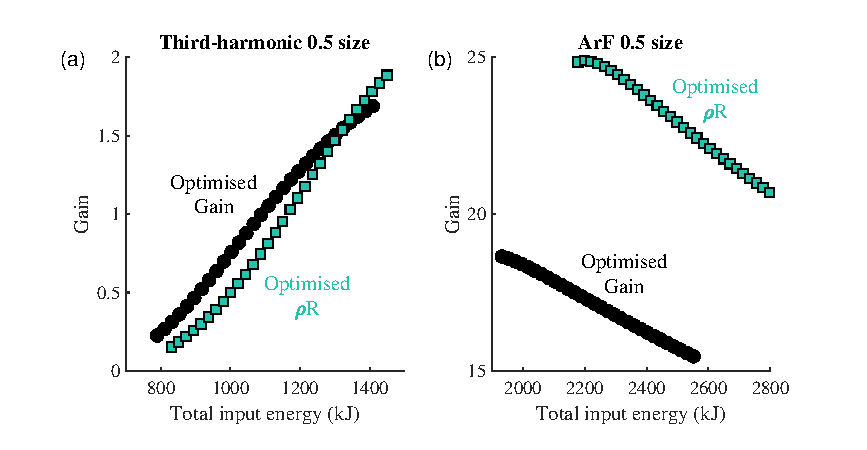
\includegraphics{figures/FurtherSims/OptimisedRhoR.eps}
\caption{Estimated gain vs total input energy for the 0.5 sized capsules optimised for gain (black) and areal density (teal), for a third-harmonic (a) and ArF (b) laser driver.}
\label{fig:OptimisedRhoR}
\end{figure}

The gain for the smaller of the two capsules, seen in Figure \ref{fig:OptimisedRhoR}(a), behaved as predicted. It can be seen that at low amounts of heating energy the `optimal gain' capsule outperforms the `optimal areal density' version. However, as the heating energy is increased further, the `optimal areal density' capsule begins to perform better, producing a higher gain than the `optimal gain capsule'. The `optimal gain' capsule begins to saturate earlier - this makes sense, since it has a lower areal density and a higher temperature, and so the temperature stops being the limiting factor much earlier than for the `optimal areal density' version.

A number of factors mean that the data in Figure \ref{fig:OptimisedRhoR}(b) is more complicated to analyse. Firstly, the optimisation procedure in this case gave an `optimal areal density' capsule at a higher laser energy than the `optimal gain' capsule (recall that this is the optimal capsule for a given radius - and not necessarily a given drive energy). The higher laser drive meant that the capsule gain was also higher, hindering useful comparison between the two capsules \footnote{This also indicates, as explained earlier, that the optimisation is not exhaustive - as there is clearly a design for this capsule radius with a higher gain than that initially optimised.}. As seen in Figure \ref{fig:OptimisedRhoR} (b), the gain is therefore higher for all amounts of deposited energy. Secondly, the much higher gain of this capsule means that the auxiliary heating in both cases does not lead to significant increases in gain, as discussed in Section \ref{sec:auxiliary-heating-of-high-gain-capsules}. However, qualitative differences are still visible - although heating adds little benefit in either case, while the `optimal gain' capsule sees gain decrease for all heating energies, there is a small increase in gain for the `optimal areal density' capsule for low amounts of heating. This is confirmed by the relative yield amplification (not plotted), which shows a greater relative increase for the `optimal areal density' capsule at low energies.

\subsection{Limitations and suggested future direction}

As stated previously, the simulations presented here are an initial investigation of the effects of such a heating scheme. They do not simulate the heating scheme itself, and thus high accuracy should not be expected. However, they indicate a promising level of performance, and suggest that further investigation of this heating process in more detail could be useful. This includes simulations of the full heating process using Vlasov-Maxwell and particle-in-cell codes, along with multi-scale modelling which can integrate the results from such codes into a fluid simulation. These are directions that are under further investigation within our group.

Another limitation of this work is the lack of accuracy to which the efficiencies for the generation and transport of the electron beams are known. These efficiencies are vital for accurate estimates of the implosion gain, and so should be determined if such a scheme is to be pursued.

A final potential limitation of this approach are the high short-pulse laser energies required. These are significantly higher than the short-pulse energies available at current facilities, and are similar to those necessary for fast-ignition schemes \cite{Strozzi2012}. Again, this an an initial investigation of this approach, which is focussed on whether such a scheme may be worthwhile rather than the practical aspects of achieving it. However, recent developments such as plasma beam combiners \cite{Kirkwood2018,Kirkwood2018a} may offer a route through which short-pulse laser energies could be increased in the future to the levels required \cite{KirkwoodPersonalComm}. Plasma beam combiners utilise non-linear scattering interactions within plasma-based optical components to produce a single laser output from multiple input beams, achieving a much higher intensity than is possible with conventional optics. It is hoped that continued development of this approach, and of short-pulse laser technology more generally, may enable the energies required for such a scheme.

\subsection{Subsequent developments of the auxiliary heating technique} \label{sec:AuxHeatingDevlopments}
Since this work was performed, there have been further developments in understanding this technique which affect how it would be applied; these are described in \cite{Lee2023}. This is not my work (it was performed by Jordan Lee, Rusko Ruskov, and Heath Martin) - but it was performed following the promising results shown here, and is included to ensure that this section covers the most up-to-date description of this process.

In the previous discussions, the heating scheme was assumed to require two overlapping electron beams. This was the setup proposed in \cite{Ratan2017}; the highest growth rates for the instabilities was seen at the overlap of these beams, and it was expected that this would therefore be where the most significant heating occurred. Having two beams in this way allowed for control over where the energy would be deposited, and by overlapping them in the hotspot deposition of electron energy into the centre of the implosion could be achieved. However, these new results instead discovered that there is no benefit to using two beams; the growth of the instabilities quickly saturate, and thus two beams provides no benefit over one. The heating occurs along the beam according to the plasma conditions at each point, and thus the position of the energy deposition cannot be controlled in this way.

Simulations of an electron beam incident on the capsule around the bang-time found that the vast majority of the energy is deposited at the edge of the hotspot. The electron beam passes through the cold, dense shell with very little absorption, but is absorbed effectively as soon as it reaches the high temperature material. This is different to the simulations here, where the energy deposition was assumed to be uniform over the central regions in the simulation. Updated versions of these HYADES simulations (performed by Jordan Lee) accounted for this, instead depositing the electron energy in a thin shell (of appropriate thickness) around the hotspot. It was found that these actually slightly improved the performance\footnote{It is suggested that this is because the material at the edge of the hotspot is likely slightly higher density but colder - and thus the heating has more of an effect}. This assumes that the heating is spherical whereas in fact this would only occur in the direction of the beam, and 2D simulations are thus required to investigate this in further detail.

\section{Conclusions}
This chapter expanded upon the results of the previous simulations in a number of different ways. Firstly, two potential limitations of the previous work were explored. The impact of the EOS used to describe the wetted-foam layer was investigated through simulations in the alternative 1D code HELIOS, where a PropacEOS `mixed-EOS' table could be used which accounted for the presence of the CH foam. This investigation was limited (due to the need to use an alternative code, and the lack of alpha-heating in HELIOS), but suggested that using a more accurate EOS for the foam layer could potentially decrease performance by around 30\%, which is comparable to other results published in the literature. Secondly, surrogate `hydrodynamic equivalent' implosions were optimised for a number of capsules, and displayed equivalent hydrodynamic performance to the main implosions. This provides a way that the results of the previous chapter (and the low-instability nature of the regime) could be explored in room-temperature experiments.

The impact of alternative laser drivers on implosions in this regime were then explored. It was demonstrated that switching from a third-harmonic Nd:glass laser to a higher frequency laser (ArF in this work) could lead to substantial increases in fusion performance for a given energy. A `two-colour' laser sequence was also proposed, which would allow some of the performance benefits of higher frequency laser energies to be obtained, while allowing the bulk of the energy to be provided by the more mature Nd:glass technology.

Finally, the effect of auxiliary heating on a number of these implosions was simulated. It was found that such a technique could potentially be used to significantly improve the fusion performance of a range of capsules. The increase on gain was also estimated to be significant, but this is highly dependent on how efficiently electron beams can be generated and their energy deposited into the hotspot. Further simulation identified that the impact of such a scheme is significantly decreased as the yield of the unheated implosion increases, suggesting that auxiliary heating is more useful for helping sub-ignition capsules to ignite rather than improving the gain of already well-performing capsules. 





